\documentclass[a4paper,12pt]{article}
\usepackage{blindtext}
\usepackage[utf8]{inputenc}
\usepackage{graphicx}
\usepackage{array}
\newcolumntype{L}{>{\raggedright\arraybackslash}m{8cm}}

\begin{document}
\begin{titlepage}
\center

\textsc{\LARGE Software Requirements Specification}\\[1.5cm]
\textsc{\Large Project: NavUP}\\[0.5cm]
\textsc{\large Team: Wheat}\\[0.5cm]

\begin{minipage}{0.4\textwidth}
\begin{flushleft} \large
\emph{Author(s):}\\
Xolo \textsc{Dandashe}\\
Mia \textsc{Gerber}\\
Hlengekile \textsc{Jita}\\
Brian \textsc{Ndung'u}\\
Nathan \textsc{Ngobale}\\
Takalani \textsc{Sigama}\\
\end{flushleft}
\end{minipage}
~
\begin{minipage}{0.4\textwidth}
\begin{flushright} \large
\emph{Student number(s):} \\
14245681\\ % Student number
15016502\\
14077893\\
15322913\\
15110045\\
14166365\\
\end{flushright}
\end{minipage}\\


\includegraphics[width=\textwidth]{images/up_logo.jpg}

{\large University of Pretoria, Department of Computer Science}\\[0.5cm]
{\large 24 February 2017}\\[3cm]

\vfil
\end{titlepage}

\newpage
\tableofcontents
\newpage

\section{Introduction}
\subsection{Purpose}
The purpose of this Software Requirements Specification(SRS) document is to provide a high level specification of the NavUP system. This document will fully describe the NavUP systems behaviour by detailing its functional and non-functional requirements. The intended audience of the document is all parties that will be involved in the project from the planning to the testing phase, this includes, designers, developers, users and more.
\subsection{Scope}
The system to be developed is called \textit{\textbf{NavUP}}. NavUP is a Navigation system for the University of Pretoria. Hence the name NavUP, Navigation UP. \\

NavUP will help numerous people who partake in activities on campus. This includes students, lecturers, workers and guests on campus. The system will not only help them maneuver around campus but also get them better acquainted with numerous aspects of the UP campus. The main task of NavUP will be providing a navigation system for the UP campus. This includes identifying locations, identifying points of interest and places where activities are taking place and providing directions to those places. This can be classes, events that take place on campus, and transportation routes such as the UP buses drop off and pick up locations, restaurants and shops on campus.

In addition the system should also be able to determine optimal routes for users to take based on their preferences as well as by avoiding pedestrian traffic, which is a common occurrence on campus. To further enhance the experience of users of the system, additional features, such as including the users campus timetable and providing directions to locations at scheduled times and counting their number of steps per day and comparing it to other users, will be included. 

The system will interface with other systems in order to achieve its purpose. These systems are namely the WiFi system currently available at UP.

\subsection{Overview}
The rest of the SRS document is organized as follows, firstly we provide an overall description which is an overview of the NavUP system. This describes the NavUP product as a whole and gives a brief description of its various interfaces and requirements, its functions, the users of the system as well as constraints and assumptions that will affect the system. Secondly we describe the software requirements of the system. This includes both the functional and non-functional requirements.

\section{Overall Description}
\subsection{Product Perspective}
\subsubsection{System Interfaces}
The NavUP will have the following system interfaces as shown in the image below,\\
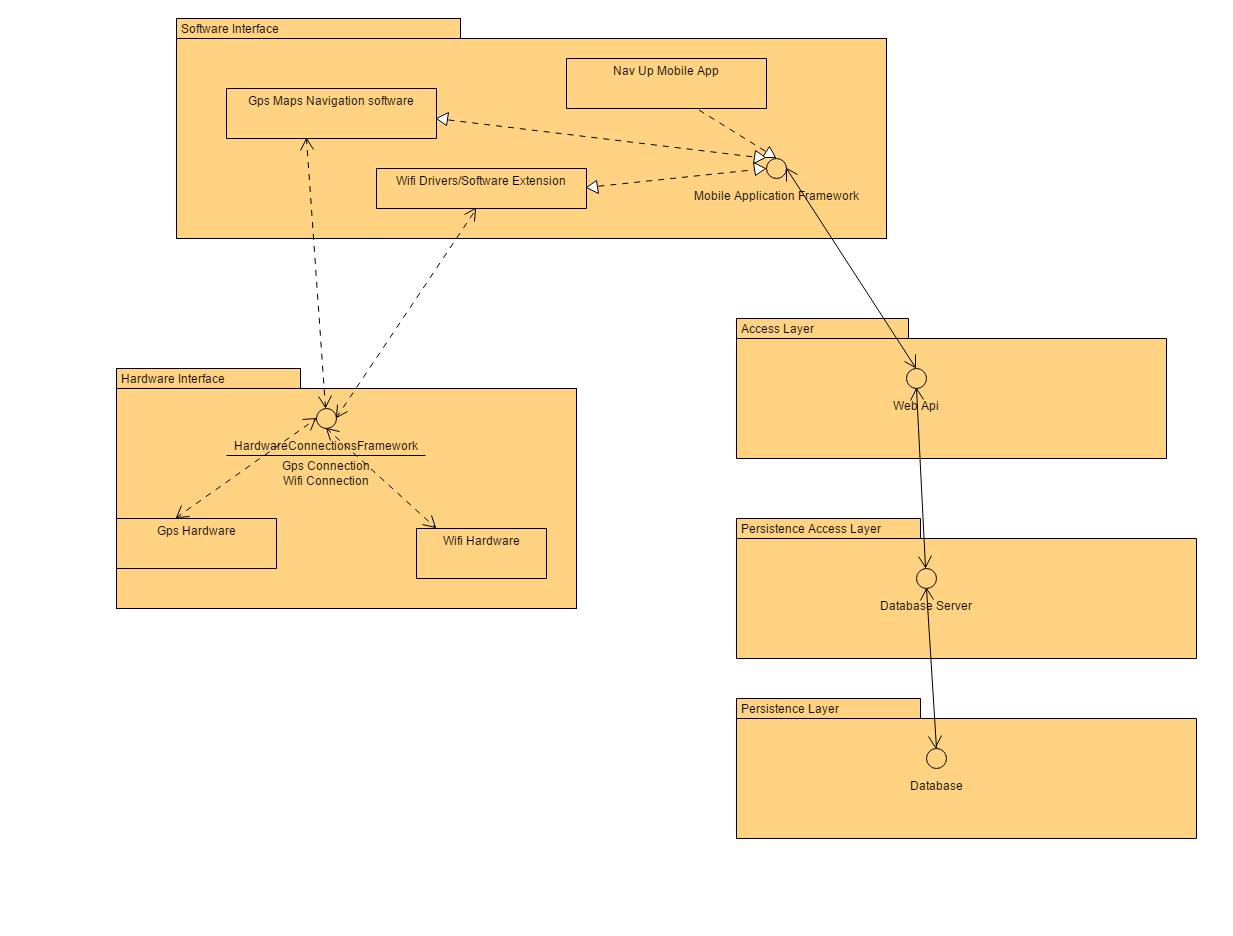
\includegraphics[width=\textwidth]{images/system_interface.png}
\textbf {Client Interface}\\
Users of the system will use a mobile application which requires a mobile device. This hardware device will either be a smart phone or a tablet and will need to have GPS and WiFi capabilities. On this device we will run an application which is our software interface which will either be the Web, Android or iOS application. These applications will access the GPS software and WiFi of the phones and interact with the server where most functionality will take place before the results are pushed back to the user.\\
\textbf{Web Server}\\
The Web Server will handle the back-end operations of the system. This will include the business processes and the CRUD database operations necessary to provide the users with the functionality. The Web Server will also be responsible for triangulating WiFi signals to pinpoint locations and any other  back-end operations \\
\textbf{Database}\\
The database will be responsible for storing all necessary persistent information. This will include but is not limited to location data, WiFi router data and user data.
\subsubsection{User Interfaces}
For this application, mobile devices like smart phones and tablets will be used. This will serve as the interface between the user and the system. Mobile applications, Android and iOS, and a Web Application will be designed for these devices, these applications will provide the users with a Graphical User Interface(GUI). A variety of screens will be shown to the user in order to provide them with information and allow them to interact with the NavUP system. These screens will be designed to give them the best user experience possible. Following, we give mock-ups of the user interface and describe some of the interactions the user should be able to make with the system. 

The user will be able to set their starting position either by setting it themselves or by use of the system's ability to determine their current position. This is demonstrated in the mock-up shown in (fig.1), the user can use this interface to set a destination and also use their previously set/visited destinations. 
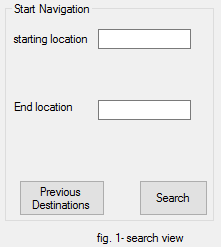
\includegraphics[width=\textwidth]{images/user_one.PNG}
Once the user is ready to search they are transferred to the screen displayed by the mock-up in (fig 2) where they can choose their desired route. Options are given to the user to select which route they prefer. They will also be given an option to get an optimal route that will  take into consideration user preferences and get the user to their destination the quickest and shortest way possible with the least traffic. Once the route is selected the user can choose to begin the navigation.
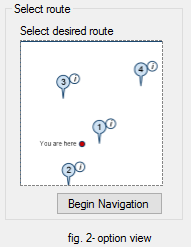
\includegraphics[width=\textwidth]{images/user_two.PNG}
A visual representation of the location of the user is given while they are en-route to their destination as show in the mock-up in (fig 3). Push notifications are sent to the user to let them know which direction should take. Total steps, distance and time taken to reach their destinations is tracked. These statistics are used to give the user goals to achieve. This is shown in the mock-up in (fig 4). A timetable integration feature will also be included which will give the user directions to classes at appropriate times, as shown in the mock-up in (fig 5).
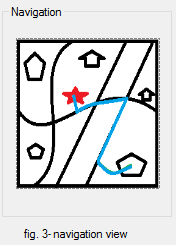
\includegraphics[width=\textwidth]{images/user_three.PNG}
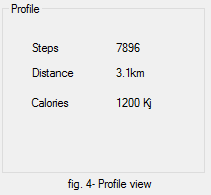
\includegraphics[width=\textwidth]{images/user_four.PNG}
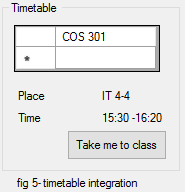
\includegraphics[width=\textwidth]{images/user_five.PNG}

\subsubsection{Hardware Interfaces}
The minimum hardware device required mainly is a mobile device either a cellphone or a tablet, that has WiFi, GPS and Internet connectivity capabilities. The system will be run using iOS and Android applications on the mobile devices. For best results with Apple devices they should be running iOS 8 or newer. For best results with other smart phones, they should be running Android version 5.0 or newer. 
\subsubsection{Software Interfaces}
The NavUP application communicates with the connected WiFi router in order to get geographical information about where the user is located and then visually represents it on the user's device. Once the current location is found, the application waits for the user to input a target destination then starts to calculate routes. 

During calculation all possible routes are determined by discerning pathways, checking most traveled route and checking pedestrian traffic. The user is then given the option to select the route they want to take, once the route is selected then navigation begins. Directions are given to the user as they are en-route and their walking statistics are recorded for their profile.
\subsubsection{Communications Interfaces}

\subsubsection{Memory}

\subsubsection{Operations}

\subsubsection{Site Adaption Requirements}

\subsection{Product Functions}
\begin{table}[!htbp]
\centering
\footnotesize
\label{tab:table 2.2}
\bgroup
\def\arraystretch{1.3}
\begin{tabular}{|L|L|}
\hline
FUNCTION & DESCRIPTION 
\\
\hline
Corrects/recalculates the path if the user is not following the route correctly. & If the user takes a wrong turn, the application will send a push notification to the user’s device, telling them that they are no longer on the correct route. The user can then either choose to recalculate the route and follow the new path or they can ask to be directed back to the original path. 
\\
\hline
Users can search for a building/location and the system will find it. & The name that the user requested can be mapped to a physical location on the UP campus. (The coordinates of specific buildings are associated with the name of the building)
\\
\hline
The user can specify a current location and destination using the search facility. & The current location and destination are saved so that it can be used to determine the route later on. 
\\
\hline
The user can use parameters so that the application can choose the optimal route for their purposes. & The application will provide several routes that the user can take to arrive at their destination, then choose from the routes generated the path that matches the criteria given by the user e.g. “shortest route” or “route that has a bathroom along the way”
\\
\hline
The application gives step by step directions on how to reach your destination & The application in real time tracks where the user is currently walking and then gives them instructions either as push notifications or audio when it is needed so the user stays on the plotted route, for example "turn left" or "take the stairs to the fourth floor". 
\\
\hline
The user can put their schedule into the application and it will generate a route for the whole day & The application will use your personalized timetable to determine a path that has every class you are going to that day along the route so that you don’t have to continually generate routes.
\\
\hline
The application tracks distance walked & You will get daily/weekly/monthly push notifications informing you of how far you have walked since a certain point in time (you can specify when the app should start calculating distance.)
\\
\hline
The application tracks which users have walked the furthest in a specific day/week/month. & The distance data from all users will be consolidated and a leader board will be created showing the top 5 students.
\\
\hline	
\end{tabular}
\egroup	
\end{table}
\subsection{User Characteristics}
\begin{itemize}
\small
\item Users will be both male and female
\item Users are university students ranging in age from 18 to 25
\item Users come from a vast array of different cultural and economic backgrounds
\item Users have graduated high school and have a median level of literacy
\item Users communicate in English using UK grammar and spelling conventions.
\item Users have used mobile devices before and are familiar with touchscreen interfaces
\item Users understand the basic concept of a wireless network and how to connect to it using a mobile device
\item Users will be both new students (no prior knowledge of the campus) and existing students (possess existing knowledge of campus)
\item Users might have disabilities, developers need to be conscious of this when designing the application. 
\end{itemize}
\subsection{Constraints}
\paragraph*{What restrictions will affect development?} 
The project requires that the application be implemented using the WiFi network on campus to determine the location of users, but because the signal strength and coverage of the network is not uniform across campus, this can severely impact the accuracy of the application and how useful it will end up being.
\\
Continuing on from the previous constraint, we can assume that because there is not WiFi available in every single part of campus, sometimes the application will have to revert to using mobile data. Students will be using the application which means our application needs to use minimal mobile data. Designing data transfer that does not use a lot of mobile data is difficult and will require us to restrict the amount of real-time data transfer that is done by the application or to implement it in a way that means they are able to use the application offline for short periods of time.  
\\
The experience of the development team may also end up becoming a constraint, the amount of features and functionality we are able to deliver on will depend largely on our technical skill level and whether we are able to come up with elegantly simple solutions.
\\
We need to ensure that this application is deployed on all mobile platforms for all mobile devices (phones, tablets, laptops etc) this means we are unable to use platform specific technologies which limits the amount of solutions we will be able to produce. 
\\
User privacy needs to be taken into account as a constraint on development. Some historical data about the user will need to be stored, but the type of data we are allowed to store will dictate which functionality we are able to bring about in the application. For example, instead of showing you your 5 most visited places, the application will only tell you how many steps you've taken in a day. 
\\
\subsection{Assumptions and Dependencies}
\begin{enumerate}
\item We are assuming that users will have the WiFi setting on their phones enabled at all times, our entire navigation system depends on this assumption because checking how the user's device connects to different routers as they move through campus is critical to determining their current location. 
\item We are assuming that the location of every WiFi router in the network is known and has been mapped onto a schematic of the Hatfield campus. We need to be able to locate the router that a user is connected to.
\item To generate a heat map of the traffic conditions on campus (where the highest concentration of people currently are) we will need to assume that all students on campus both have the application downloaded and running while they are moving around on campus.
\item All possible solutions outlined in this document will work on the assumption that we have not been given any limit on the size of our database or the capacities of the server that will be used.
\end{enumerate}

\section{Specific Requirements}
\subsection{External Interface Requirements}

\subsection{Functional Requirements}

\subsection{Performance Requirements}

\subsection{Design Constraints}

\subsection{Software System Attributes}

\subsection{Other Requirements}

\section{Appendix}
\subsection{Glossary of terms}
%Explanations of terms
%Definitions, Acronyms, Abbreviations
\subsection{References}
%Software Engineering textbook, more if any
\section{Index}

\end{document}